\section{Обсуждение результатов}
% ── Таблица: метрики ──────────────────────────
\begin{table}[H]
  \centering
  \small
  \setlength{\tabcolsep}{4pt}
  \begin{tabularx}{\textwidth}{@{} X ccccccc @{}}
    \toprule
    \textbf{Модель} &
    \textbf{STS ($\rho$)} & \textbf{20NG (Acc)} & \textbf{20NG (F1)} &
    \textbf{ARI} & \textbf{Sil.} & \textbf{MRPC (F1)} \\
    \midrule
    LSA $k{=}300$
    & 0.56 & 0.673 & 0.658 & 0.17 & 0.047 & 0.817 \\
    \midrule
    \textbf{MiniLM-L6-v2}
    & \textbf{0.82} & \textbf{0.703} & \textbf{0.688}
    & \textbf{0.37} & \textbf{0.066} & \textbf{0.835} \\
    \bottomrule
  \end{tabularx}
  \vspace{1mm}
  \caption{Экстринсивные метрики.}
  \label{tab:extrinsic_results}
\end{table}

\begin{table}[H]
  \centering
  \small
  \setlength{\tabcolsep}{4pt}
  \begin{tabularx}{\textwidth}{@{} X cccc @{}}
    \toprule
    \textbf{Модель} &
    \textbf{PR} & \textbf{ER} & \textbf{IS} & \textbf{HS} \\
    \midrule
    LSA $k{=}300$
    & 198.60 & 284.93 & 0.0120 & 3.54 \\
    \midrule
    \textbf{MiniLM-L6-v2}
    & 117.85 & 312.97 & 0.0011 & \textbf{1.77} \\
    \bottomrule
  \end{tabularx}
  \vspace{1mm}
  \caption{Интринсивные метрики.}
  \label{tab:intrinsic_results}
\end{table}


\paragraph{Семантическое сходство (STS).}
\texttt{all-MiniLM-L6-v2} существенно превосходит LSA по корреляции Спирмена
($\rho = 0.82$ против $0.59$ при $k = 500$). Кривая LSA
монотонно возрастает на всём диапазоне $k \in \{50, \ldots, 500\}$ и не
выходит на плато (рис.~$\ref{fig:sts_vs_k}$), что свидетельствует об отсутствии
верхней границы в исследованном диапазоне. Тем не менее, ограничение
модели (\enquote{мешок слов}) принципиально: явления, определяющие
семантическое сходство в STSb (порядок слов, отрицание и
полисемия) полностью игнорируются TF-IDF вне зависимости от размерности $k$.

% ── График: STS ρ vs k ─────────────────────────────────────
\begin{figure}[H]
  \centering
  \begin{tikzpicture}
    \begin{axis}[
        width=\textwidth,
        xlabel={Размерность $k$},
        ylabel={Spearman $\rho$},
        xmin=0, xmax=550,
        ymin=0.3, ymax=0.9,
        xtick={50,100,200,300,500},
        grid=major,
        grid style={dashed, gray!80},
        legend pos=south east,
      ]
      \addplot[blue, mark=square*, thick] coordinates {
        (50,  0.4074)
        (100, 0.4553)
        (200, 0.5262)
        (300, 0.5635)
        (500, 0.5944)
      };
      \addlegendentry{LSA}

      \addplot[red, dashed, thick, domain=0:550] {0.820};
      \addlegendentry{\texttt{all-MiniLM-L6-v2}}
    \end{axis}
  \end{tikzpicture}
  \caption{Зависимость STS Spearman $\rho$ от размерности $k$.}
  \label{fig:sts_vs_k}
\end{figure}


\paragraph{Тематическая классификация (20NG).}
Разрыв между моделями на задаче классификации значительно меньше, чем на STS:
\texttt{all-MiniLM-L6-v2} превосходит LSA $k=300$ лишь на $0.03$ по F1-macro
($0.688$ против $0.658$). Это свидетельствует о том, что тематика
успешно улавливается линейной моделью при достаточно большой
размерности.

\paragraph{Кластеризация (20NG).}
Наибольший разрыв между моделями обнаруживается именно в задаче кластеризации:
$ARI = 0.37$ у \texttt{all-MiniLM-L6-v2} против $ARI = 0.17$ у
LSA при $k = 300$. Это наиболее информативный
результат эксперимента, поскольку кластеризация проводится без разметки и
оценивает геометрическую структуру пространства напрямую.

% ── График: тепловая карта MiniLM ───────────────────────────
\begin{figure}[htbp]
  \centering
  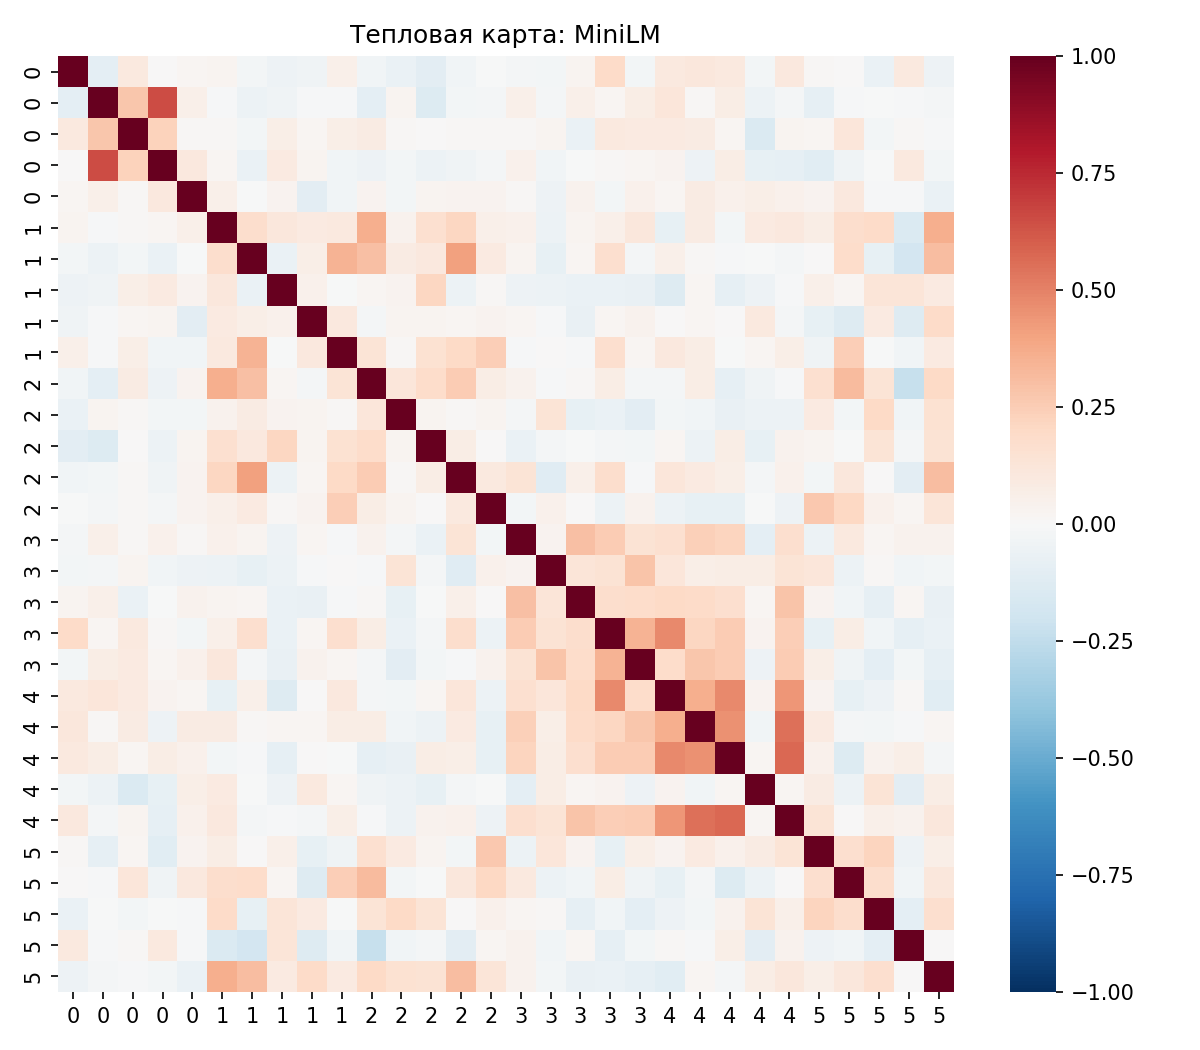
\includegraphics[width=\textwidth]{cosine_heatmap_Тепловая.png}
  \caption{Тепловая карта косинусного сходства \texttt{all-MiniLM-L6-v2}
  (20NG, 6 классов). Блочная структура соответствует $ARI = 0.37$.}
  \label{fig:heatmap_minilm}
\end{figure}

\paragraph{Обнаружение парафраз (MRPC).}
LSA при $k = 300$ ($F1 = 0.817$) незначительно уступает
\texttt{all-MiniLM-L6-v2} ($F1 = 0.835$). Малый разрыв объясняется
природой датасета: MRPC содержит преимущественно перефразировки
новостных предложений, в которых ключевые слова совпадают~--- такой
лексический сигнал оказывается достаточным для модели \enquote{мешка
слов}.

\paragraph{Изотропия и прикладное качество.}
Наиболее неожиданным результатом является сочетание крайне низкой изотропии
\texttt{all-MiniLM-L6-v2} ($IS = 0.001$) с высоким результатом на
прикладных задачах. Дисперсия в пространстве трансформера
сосредоточена в нескольких доминирующих направлениях, тогда как
остальные компоненты несут минимум информации. Таким образом, $IS$
является индикатором геометрической равномерности, однако не отражает
эффективность модели на прикладных задачах.

\paragraph{Effective Rank.}
$ER(\text{LSA}, k=300) = 284.93$ сопоставим с $ER(\texttt{MiniLM}) =
312.97$, при этом $PR(\text{LSA}) = 198.60$ превышает
$PR(\texttt{MiniLM}) = 117.85$. TruncatedSVD по конструкции отбирает
$k$ компонент с наибольшими сингулярными числами, которые в рамках
усечённого подпространства остаются относительно равномерными. Данный
результат демонстрирует, что высокие PR и ER не являются достаточным
условием семантического качества.

% ── График: спектр сингулярных чисел ────────────────────────
\begin{tikzpicture}
  \begin{axis}[
      xlabel = {Компонента},
      ylabel = {Нормализированное сингулярное число},
      xtick = {1, 25, 50, 75, 100},
      ymin=0, ymax=0.82,
      grid =both,
    ]
    \addplot table[x=i, y=lsa] {figures/spectrum.dat};
    \addlegendentry{LSA}

    \addplot table[x=i, y=bert] {figures/spectrum.dat};
    \addlegendentry{BERT}

  \end{axis}
\end{tikzpicture}

